% !Tex root=main.tex

\section{AFA}

This sections introduces \emph{succinct alternating finite automata} (AFA) as they are used in \sloth and explains why the authors of \sloth opted to use this model of computation instead of other possible models.
Indeed, AFA have no additional power in expressiveness over \emph{non deterministic finite automata} (NFA), thus AFA are equivalent with NFA and regular languages.

In section \ref{sec:preliminaries} we noted that we are interested in unsatisfiability of string constraints, as we translate the string constraint into an AFA this will translate into solving emptiness for the corresponding automata.
Remark that solving emptiness for NFA is NLOG-SPACE-complete and a linear search over the state space is enough to check if an NFA is empty.
For AFA, however, deciding emptiness becomes PSPACE-complete, so one might ask why it is preferred to use AFA over NFA.
Essentially, this boils down to two major reasons:
\begin{enumerate}
\item Translating an AFA to an NFA requires a subset construction, thus an NFA equivalent to an AFA is exponentially bigger. Exploring the state space of the NFA for the emptiness check is still running in linear time, however, linear in the exponentially sized NFA.

\item Boolean combinations on AFA is significantly cheaper than on NFA. The intersection of two AFA $A_1$ and $A_2$ would be of the size $A_1 + A_2$ while using NFA the size would be in $O(|A_1| \cdot |A_2|)$. Many of those boolean combinations are needed when translating the formula to an AFA, as the translation starts with a formula and ends up with only one AFA.
\end{enumerate}

Thus, AFA being exponentially smaller than NFA and allowing more efficient way of applying boolean combinations, makes using them more attractive.
In the following the syntax of AFA is introduced, afterwards the notion is illustrated on a small example.

\paragraph*{Bitvectors encoding the alphabet.} The automata will work on \emph{bit vectors} instead of an alphabet $\Sigma$ which is usually used when introducing AFA or NFA.
This is a further step in shrinking the size of the automata. Bit vectors are functions $\mathcal{B}: V \mapsto \mathbb{B}$, where $V$ is a finite, totally ordered set of bit variables.
\begin{example}
Given an alphabet $\Sigma = \{a,b,c,d\}$, a set $V = \{v_0,v_1\}$ can be introduced to encode $\Sigma$ as follows. The symbol $a$ is encoded as $\lnot v_1 \wedge \lnot v_0$, $b$ as $\lnot v_1 \wedge v_0$, $c$ as $ v_1 \wedge \lnot v_0$, and $d$ as $v_1 \wedge v_0$.
\end{example}
\paragraph*{Syntax of AFA.} A succinct alternating automata is a quintuple $\mathcal{A} = (V,Q,\Delta, I, F)$. $V$ is a set of variables which is used to encode an alphabet $\Sigma$, $Q$ is a finite set of states, the transition relation $\Delta : Q \mapsto \mathbb{F}_{V \cup Q}$ maps every state to a formula over the variables and the states. 
The state variables must occur positively in the formula which means they appear under an even amount of negations.
The initial formula $I \in \mathbb{F^+_Q}$ is a positive formula and the final formula $F \in \mathbb{F^-_Q}$ is a negative formula over the state variables.
Let $w = b_1 \dots b_m$, be a word where each $b_i$ encodes the $i$-letter of $w$. A \emph{run} $\rho$ of the AFA $\mathcal{A}$ is a sequence $\rho = q_0b_1\dots b_m q_m$ where $q_i \subseteq Q$ for every $0 \leq i \leq m$ and $b_i \in \mathcal{P}(V)$ for every $1 \leq i \leq m$ and $b_i \cup p_i \vDash \bigwedge_{q\in pi_{i-1}} \Delta (q)$ for every $0 \leq i \leq m$.
A run $\rho$ is accepting if and only if $q_0 \models I$ and $q_m \models F$.
Note, that the authors used a sequence to describe a run, intuitively you can think of a run as a tree rather than a sequence as follows. The root node is the empty symbol $\epsilon$ and $\epsilon$ has a $k$ children $x_1,\dots x_k$ for some $k \leq |Q|$ such that $\{x_1,\dots, x_k\} \models I$. Afterwards, you apply this procedure of unrolling the transition relation $\Delta$ on all children nodes as depicted in Figure \ref{??}.
The run is accepting if for all leaf nodes $l_i \models F$.
\begin{figure}
\centering
	\begin{tikzpicture}
		\begin{scope}[every node/.append style={font=\strut\footnotesize}]
			\node (0) at (0, 0) {$\epsilon$};
			\node (1) at (-1.5, -.75) {$x_1$};
			\node (2) at (-0.5, -.75) {$\vdots$};
			\node (3) at (0.5, -.75) {$\vdots$};
			\node (4) at (1.5, -.75) {$x_k$};
			\node (6) at (-1.5, -1.5) {$\vdots$};
			\node (7) at (-0.5, -1.5) {$\vdots$};
			\node (8) at (0.5, -1.5) {$\vdots$};
			\node (9) at (1.5, -1.5) {$\vdots$};
			\node (10) at (-1.5, -2.25) {$l_2$};
			\node (11) at (-0.5, -2.25) {$\vdots$};
			\node (12) at (0.5, -2.25) {$\vdots$};
			\node (13) at (2, -2.25) {$l_{m}$};
			\node (14) at (-2, -2.25) {$l_1$};
			\node (16) at (-1, -2.25) {$\vdots$};
			\node (17) at (1, -2.25) {$l_{m-1}$};
		\end{scope}

		\draw (0) -- (1) (0) -- (2) (0) -- (3) (0) -- (4)(1) -- (6) (2) -- (7) (3) -- (8) (4) -- (9) (6) -- (10) (7) -- (11) (8) -- (12) (9) -- (13) (6) -- (14)  (9) -- (17) (6) -- (16);
	\end{tikzpicture}
		\caption{A run tree for an AFA. The input symbols are omitted in this tree to make it more readable.} \label{fig:decision-tree}
\end{figure}

\begin{example}
Consider AFA $\mathcal{A} = (V, Q, \Delta, I, F)$ over the alphabet $\Sigma = \{a,b\}$. 
The language of $\mathcal{A}$ is $a^*$.
Let $V = {v_0}$, where $a$ is encoded as $\lnot v_0$ and $b$ as $v_0$.
The set of states is defined as $Q = \{q_0,q_1\}$, the initial formula as $I = q_0$ and the final formula as $F = \lnot q_1$ which is equivalent to $q_0$.
Finally, the transition relation is defined as follows:
\begin{align*}
\Delta(q_0)& = q_0 \wedge q_1 \wedge v_0 \vee (q_0 \vee q_1) \wedge \lnot v_0\\
\Delta(q_1)& = q_1 \wedge \lnot v_0
\end{align*}
\begin{figure}
\begin{tikzpicture}
\node[state, initial, accepting] at (0,0)(q1) {$q_0$};
\node[state, right of=q1, xshift = 3cm](q2) {$q_1$};
\draw[->] (q1) edge[loop above] node{$\lnot v_0$} (q1)
(q1) edge[above] node{$\lnot v_0$} (q2)
(q2) edge[loop above] node{$\lnot v_0$} (q2)
(q1) edge [in=120, out=45] (q2)
(q1) edge [in=120, out=45,looseness = 8] (q1);
\draw[thick] (1,0.815) arc (40:60:1.8) node[anchor= south west]{$v_0$};
\end{tikzpicture}
		\caption{AFA $\mathcal{A}$, the conjunction $q_0 \wedge q_1 \wedge v_0$ is drawn with a thick arc which indicates that both edges need to be followed when applying this transition} \label{fig:afa}
\end{figure}


\begin{figure}
\hskip 1em
\begin{subfigure}{0.2\textwidth}
\centering
	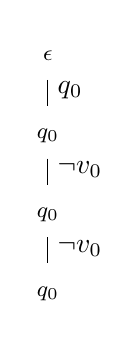
\begin{tikzpicture}
		\begin{scope}[every node/.append style={font=\strut\footnotesize}]
			\node (0) at (0, 0) {$\epsilon$};
			\node (1) at (0, -1) {$q_0$};
			\node (2) at (0, -2) {$q_0$};
			\node (3) at (0, -3) {$q_0$};
		\end{scope}

		\draw (0) -- (1) node[anchor = south west,yshift = 0.3cm]{$q_0$} (1) -- (2) node[anchor = south west,yshift = 0.3cm]{$\lnot v_0$} (2) -- (3) node[anchor = south west,yshift = 0.3cm]{$\lnot v_0$};
	\end{tikzpicture}
	\vskip 3em
		\caption{A run on the word $w_1 = aa$ on the AFA $\mathcal{A}$. Remember, that $a$ is encoded as $\lnot v_0$.} \label{fig:run-aa}
\end{subfigure}
\hskip 3em
\begin{subfigure}{0.2\textwidth}
\centering
	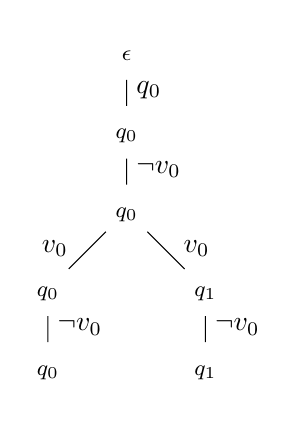
\begin{tikzpicture}
		\begin{scope}[every node/.append style={font=\strut\footnotesize}]
			\node (0) at (0, 0) {$\epsilon$};
			\node (1) at (0, -1) {$q_0$};
			\node (2) at (0, -2) {$q_0$};
			\node (3) at (-1, -3) {$q_0$};
			\node (4) at (1, -3) {$q_1$};
			\node (5) at (-1, -4) {$q_0$};
			\node (6) at (1, -4) {$q_1$};
		\end{scope}

		\draw (0) -- (1) node[anchor = south west,yshift = 0.3cm]{$q_0$} (1) -- (2) node[anchor = south west,yshift = 0.3cm]{$\lnot v_0$} (2) -- (3) node[anchor = south west,yshift = 0.3cm, xshift = -0.2cm]{$v_0$} (2) -- (4) node[anchor = south west,yshift = 0.3cm, xshift = -0.4cm]{$v_0$}
		(4) -- (6) node[anchor = south west,yshift = 0.3cm]{$\lnot v_0$} (3) -- (5) node[anchor = south west,yshift = 0.3cm]{$\lnot v_0$};
	\end{tikzpicture}
		\caption{A run on the word $w_2 = aba$ on the AFA $\mathcal{A}$. Remember, that $a$ is encoded as $\lnot v_0$  and $b$ as $v_0$.} \label{fig:run-aba}
\end{subfigure}
\end{figure}
Two runs on an AFA are shown in Figure \ref{fig:run-aa} and \ref{fig:run-aba} . Figure \ref{fig:run-aa} shows an accepting run on the word $w_1 = aa$. 
The AFA $\mathcal{A}$ has to make a non-deterministic decision on input $a$.
Thus, the AFA behaves like an NFA and it suffices to encode the run as a sequence.
The run is accepting the word $w_1$ because the run ends up in state $q_0$ which is an accepting state.
The word $w_2 = aba$, however has runs that forces the tree to have more than one branch, as depicted in Figure \ref{fig:run-aba}.
When reading the symbol $b$ in state $q_0$, the transition relation goes over to $q_0 \wedge q_1$.
This can be seen as an universal transition since now the run splits into two branches, that have $q_0$ and $q_1$ as states and both of those branches have to end up in an final state for the run to be accepting.
One of the branches ends up in $q_0$ which is an final state, however, the other branch ends up in $q_1$ which is not a final state, making this a non accepting run on the word $w_2$.
Indeed, you can easily check the all runs on the word $w_2$ are non accepting by checking all non-deterministic choices.
\end{example}

\paragraph*{Boolean Operations on AFA.} Transforming a formula into an AFA requires many boolean operations on AFA including conjunction, disjunction and complementation.
It is crucial to keep the size of the resulting AFA small and this is possible for all of those operations in term of of size of the state space.
In detail, all of the operations can be implemented in linear time and space in the size of the state space.
However, complementation contains possible sources for exponential blow-up for the transition relation which can have an impact on the emptiness check.

Given two AFAs $\mathcal{A} = (V,Q,\Delta, I, F)$ and $\mathcal{A}' = (V,Q',\Delta', I', F')$ with $Q \cap Q' = \emptyset$, the union of their languages can be constructed as $\mathcal{A} \cup \mathcal{A}' = (V,Q \cup Q',\Delta \cup \Delta', I\vee I', F\wedge F')$ and the intersection as $\mathcal{A} \cap \mathcal{A}' = (V,Q \cup Q',\Delta \cup \Delta', I\wedge I', F\wedge F')$.

The correctness of the union can be argued as follows.
One of the automata can start with the empty set of states since only one part of the initial formula has to be satisfied. 
Thus, the automata starting with the empty set of states remains in the empty set of states and satisfies the negative final formula trivially. 
The correctness of the intersection can be seen immediately because the initial condition enforces the two AFA to run in parallel while the final condition only allows runs to be accepted when both AFAs are accepting.

For the complementation the authors used a procedure proposed by D'Antoni et al. \cite{???}. 
First the AFA needs to be brought into the correct form which means simplifying the final condition and the transition relation.
Afterwards the complementation procedure is applied.

Block for the complementation and the transformation?
Block for the complementation and the transformation?
Block for the complementation and the transformation?
Block for the complementation and the transformation?
Block for the complementation and the transformation?
Block for the complementation and the transformation?
Block for the complementation and the transformation?
Block for the complementation and the transformation?
Block for the complementation and the transformation?
Block for the complementation and the transformation?
Block for the complementation and the transformation?
Block for the complementation and the transformation?

Note that this complementation contains three sources of exponential blow-up.
\begin{enumerate}
\item Simplification of final condition requires DNF
\item Simplification of transitions
\item Normalization of transitions
\end{enumerate}

The authors argue that the first blow-up does not apply here because the complementation will only be applied on AFAs obtained by Boolean operations from NFAs derived from regular expressions.
Thus, the AFA have already simple final conditions.
The other two sources of blow-ups only apply to the size of the transition relation which can have an impact on the performance when the transition relation gets to big as PDR is using the transition relation intensively in many SAT queries.
\paragraph*{Remark.} The authors of \sloth also use alternating finite transducers (AFT) to encode rational constraints. The concept of AFT is similar to AFA and AFT can be interpreted as AFA by increasing the size of the alphabet, thus, this paper will not go into further detail on AFT.
The authors of a different string solver named Qzy \cite{??} also go over automata to transition systems.
However, they use boolean finite automata (BFA) to encode their formulas.
BFA offer a linear time and space transformation for the complementation which does not increase the size of the transition relation, the size of the transition relation stays the same after complementing.
This concept, however, is only used for formulas over Regular language constraints, dropping the rational constraints which \sloth is able to solve.
\paragraph{Syntax of BFA.} A boolean finite automaton is a quintuple $B = (\Sigma, Q, I , F, \Delta)$ over an alphabet $\Sigma$. \cite{succinct rep of reg lang by boolean automata}
$Q$ is a finite set of states, $I: 2^Q \mapsto \{0,1\}$ is a boolean function which encodes the initial states and $F: Q \mapsto \{0,1\}$ is an indicator function for the final assignments.
Finally, the transition relation is relation which maps a state and a symbol to a boolean function $\Delta: Q \times \Sigma \mapsto (f_{q,a})$ where $f_{q,a}: 2^Q \mapsto \{0,1\}$.
The transition relation is applied as follows.
Given a word $w \in \Sigma^*$, $a_j \in \Sigma$, $q_i \in Q$, and a boolean function $f$.
$\Delta(q_i, \epsilon) = q_i$, is the transition relation applied on the empty word $\epsilon$.
On a single state the transition relation is applied as $\Delta(q_i, a_jw) = f_{ij}(\Delta(q_1,w),\dots, \Delta(q_n, w))$, where $f_{ij}(q_1,\dots,q_n) = \Delta(q_i,a_j)$.
On a set of states defined as a boolean function $f$ the transition relation is applied as $\Delta(f,w) = f(\Delta(q_1,w), \dots, \Delta(q_n,w))$.
The indicator function $F$ is used a an interpretation for the resulting formula, thus, a word $w$ is accepted by $B$ iff $F \vDash \Delta(I,w)$.

Informally, the difference between AFA and BFA is that AFA does computations over a set of states while BFA does computation over boolean formulas.
This allows for an easier complementation method as only the result of the formula has to be complemented instead of trying to take the complement of the set of states.
\begin{figure}[t]
\centering
	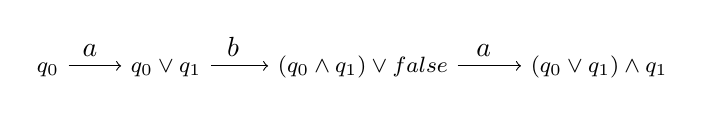
\begin{tikzpicture}
		\begin{scope}[every node/.append style={font=\strut\footnotesize}]
			\node (0) at (0, 0) {$q_0$};
			\node (1) at (1.5, 0) {$q_0 \vee q_1$};
			\node (2) at (4, 0) {$(q_0 \wedge q_1) \vee false$};
			\node (3) at (7, 0) {$(q_0 \vee q_1)\wedge q_1$};
		\end{scope}

		\draw [->] (0) -- (1) node[anchor = south east, xshift = -0.75cm]{$a$};
		\draw [->] (1) -- (2) node[anchor = south east, xshift = -1.45cm]{$b$};
		\draw [->]  (2) -- (3) node[anchor = south east, xshift = -1.25cm]{$a$} ;
	\end{tikzpicture}
		\caption{Unrolling of the transition relation $\Delta$ of the BFA $B$ on the word $w = aba$.} \label{fig:bfa-aba}
\end{figure}
\begin{example}\label{ex:bfa}
Consider BFA $B = (\Sigma, Q, I, F, \Delta)$ over the alphabet $\Sigma = \{a,b\}$. 
The language of $B$ is $a^*$.
The set of states is defined as $Q = \{q_0,q_1\}$, the initial formula as $I = q_0$ and the indicator function as $F = [q_0 \mapsto 1, q_1 \mapsto 0] $.
Finally, the transition relation is defined as follows:
\begin{align*}
\Delta(q_0,a)& = q_0 \vee q_1\\
\Delta(q_0,b)& = q_0 \wedge q_1\\
\Delta(q_1,a)& = q_1\\
\Delta(q_1,b)& = false
\end{align*}
\vskip -0.5em
An application of the transition relation of the BFA $B$ on the word $w = aba$ is shown in Figure \ref{fig:bfa-aba}.
In each step the transition relation is applied on all states $q_i$ while keeping the boolean connectives. 
The word is not accepted by the automaton since $ F \not \models q_0 \wedge (q_0 \vee q_1)$.
\end{example}
Applying boolean operations on BFA can be achieved by only manipulating the initial formula as follows. Given two BFA $B = (\Sigma, Q, I, F, \Delta)$ and $B' = (\Sigma', Q', I', F', \Delta')$. The union of their languages can be constructed as $B\cup B' = (\Sigma \cup \Sigma', Q \uplus Q' , I \vee I', F \uplus F', \Delta \uplus \Delta')$, the intersection as $B\cap B' = (\Sigma \cup \Sigma', Q \uplus Q' , I \wedge I', F \uplus F', \Delta \uplus \Delta')$, and finally the complementation as $B^{\mathit{C}} = (\Sigma, Q, \lnot I, F, \Delta)$.
The proof for the complementation can be done in the following way: 

\begin{proof}[Proof]
Given a BFA $B = (\Sigma, Q, I, F, \Delta)$ with the language $L(B)$.
\begin{align*}
w \in L(B) \iff & w \text{ is accepted by $B$}\\
\iff &F \models \Delta(I,w) \\
\iff &F \not \models \Delta(\lnot I, w) \\
\iff &w \text{ is not accepted by $B$}^{\mathit{C}} \\
\iff &w \not \in \Sigma^*~ \textbackslash~L(B) \\
\iff &w \not \in L(B^{\mathit{C}})
\end{align*}
\end{proof}

\begin{example}
Reconsider the BFA $B$ from Example \ref{ex:bfa}. Complementing $B$ gives us $B^{\mathit{C}} = (\Sigma, Q, \lnot I, F, \Delta)$. Figure \ref{fig:bfac-aba} depicts the application of the transition relation on the word $w = aba$.
You can see that the application is applied in a similar manner as in Figure \ref{fig:bfa-aba} which is on the BFA $B$, however, the formula is negated because $B^{\mathit{C}}$ starts in $\lnot I$.
$F \models \lnot ((q_0 \vee q_1) \wedge q_1)$, thus the word $w$ is accepted by $B^{\mathit{C}}$.
\end{example}


\begin{figure}
\centering
	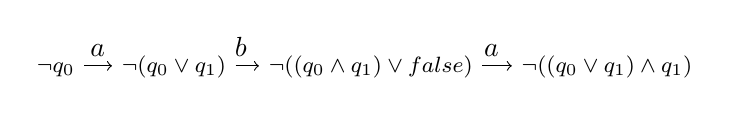
\begin{tikzpicture}
		\begin{scope}[every node/.append style={font=\strut\footnotesize}]
			\node (0) at (0, 0) {$\lnot q_0$};
			\node (1) at (1.5, 0) {$ \lnot (q_0 \vee q_1)$};
			\node (2) at (4, 0) {$\lnot ((q_0 \wedge q_1) \vee false)$};
			\node (3) at (7, 0) {$\lnot((q_0 \vee q_1)\wedge q_1)$};
		\end{scope}

		\draw [->] (0) -- (1) node[anchor = south east, xshift = -0.75cm]{$a$};
		\draw [->] (1) -- (2) node[anchor = south east, xshift = -1.45cm]{$b$};
		\draw [->]  (2) -- (3) node[anchor = south east, xshift = -1.25cm]{$a$} ;
	\end{tikzpicture}
		\caption{Unrolling of the transition relation $\Delta$ of the BFA $B^{\mathit{C}}$ on the word $w = aba$.} \label{fig:bfac-aba}
\end{figure}

Both automata models are equivalent with NFA, comprising the size needed for an NFA in a similar way.
As you can see BFAs have a very efficient complementation procedure which does not increase the size of the automaton, however, other tricks that the authors of \sloth have used might be more difficult on BFA than AFA as BFA have a completely different definition of acceptance.
Both automata models can be translated into transition systems and hardware model checkers are used to solve reachability in such transition systems.
The next section of this paper is about property directed reachability, the opted method of the authors of \sloth to solve reachability in transition systems.